\documentclass{article}
\usepackage{graphicx} % Required for inserting images
\usepackage{hyperref}
\usepackage{caption}
\usepackage{float}
\usepackage{subcaption}

\title{Robot Gripper}
\author{ \\ Abdelrahman Abdelghany - 202301000 \\ \\ Martin Rober - 202301070 \\ \\ Mostafa Sameh - 202300781 \\ \\ \\ \\ \\  }
\date{Janurary 1st, 2025}

\begin{document}

\maketitle

\newpage
\section*{Introduction}
Robot arms$^{(1)}$ are usually designed to handle a job for a human. They're usually motor operated,
and are composed of parts connected together through joints in order to mimic a human hand's movements
(although, some are much more primitive; i.e. not exhibiting the complex anatomy of a human hand).
\newline \newline
A special class of robot arms are robot grippers, which are usually primitive in shape.
\begin{figure}[h]
    \centering
    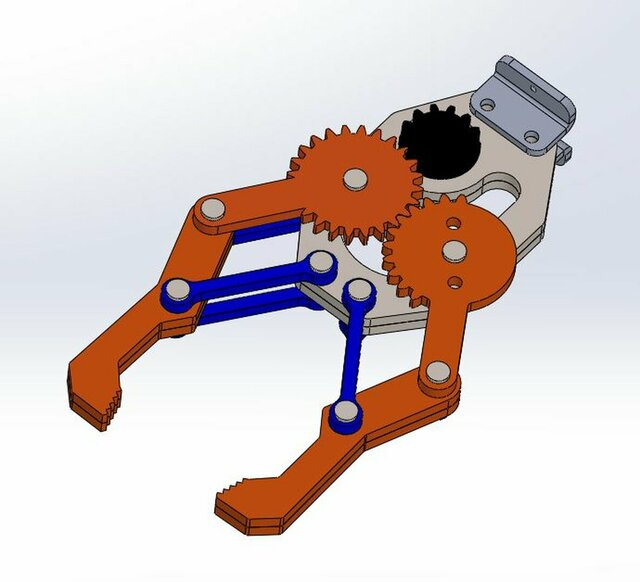
\includegraphics[width=0.5\linewidth]{Images/gear-operated_robot_gripper.jpg}
    \caption{Example of a Gear-Operated Robot Gripper}
    \label{fig:f1}
\end{figure}
\begin{figure}[h]
    \centering
    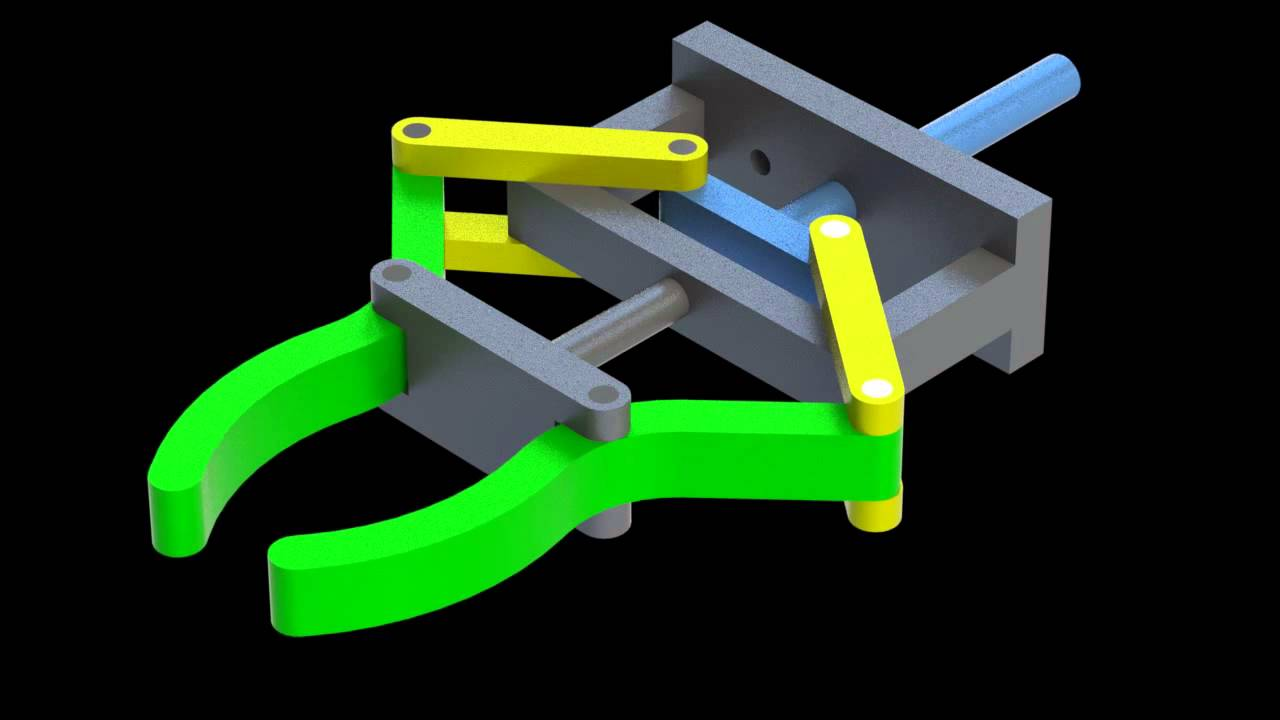
\includegraphics[width=0.5\linewidth]{Images/piston-operated_robot_gripper.jpg}
    \caption{Example of a Piston-Operated Robot Gripper}
    \label{fig:f2}
\end{figure}
\newline
Robot grippers are usually constructed using simple mechanisms, such as a gear-operated gripper,
which mainly depends on a set of gears to work, or such as a piston-operated one, which relies
on a piston to open and close the hand.
\newline \newline
Robot grippers are most often used for a simple reason; that is$^{(2)}$, a human hand is prone to tiring
and is prone to making mistakes and errors during repetitive tasks, while a robot gripper does 
not tire and operates endlessly and tirelessly. For this reason, robot grippers are sometimes used
in the industry in production lines, where routine tasks are to be performed continuously.


\newpage
\section*{Design}

\begin{figure}[H]
    \centering
    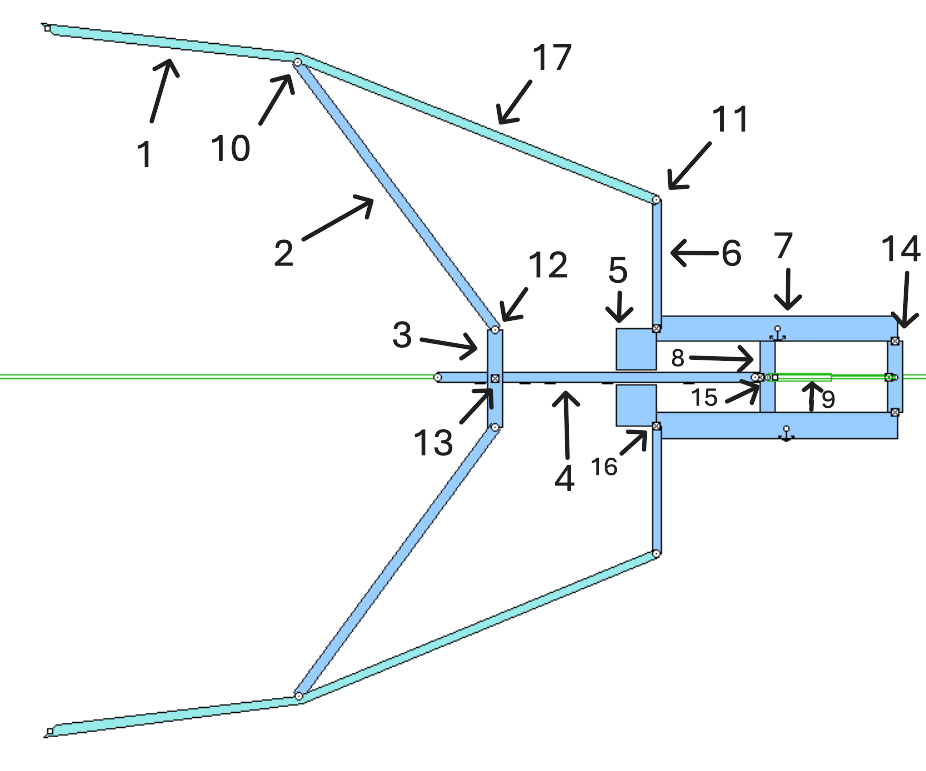
\includegraphics[width=0.7\linewidth]{Images/Design.PNG}
    \caption{Robot Gripper Design}
\end{figure}
\textbf{Member 1} $\rightarrow$ H = 0.02 m \qquad W = 0.5085 m
\newline\newline
\textbf{Member 17} $\rightarrow$ H = 0.02 m \qquad W = 0.7521 m
\newline\newline
\textbf{Member 2} $\rightarrow$ H = 0.65 m \qquad W = 0.02 m \qquad m = 1.3 kg
\newline\newline
\textbf{Member 3} $\rightarrow$ H = 0.19 m \qquad W = 0.03 m \qquad m = 0.57 kg
\newline\newline
\textbf{Member 4} $\rightarrow$ H = 0.02 m \qquad W = 0.63 m \qquad m = 1.26 kg
\newline\newline
\textbf{Member 5} $\rightarrow$ L = 0.08 m \qquad m = 0.64 kg
\newline\newline
\textbf{Member 6} $\rightarrow$ H = 0.25 m \qquad W = 0.016 m \qquad m = 0.4 kg
\newline\newline
\textbf{Member 7} $\rightarrow$ H = 0.05 m \qquad W = 0.47 m \qquad m = 2.35 kg
\newline\newline
\textbf{Member 8} $\rightarrow$ H = 0.14 m \qquad W = 0.03 m \qquad m = 0.42 kg
\newline\newline
\textbf{Member 9} $\rightarrow$ Actuator
\newline\newline
\textbf{Member 10, 11, 12}  $\rightarrow$ Pin joints
\newline\newline
\textbf{Member 13, 14, 15, 16}  $\rightarrow$ Connecting joints



\newpage
\section*{Results}

\begin{figure}[H]
    \centering
    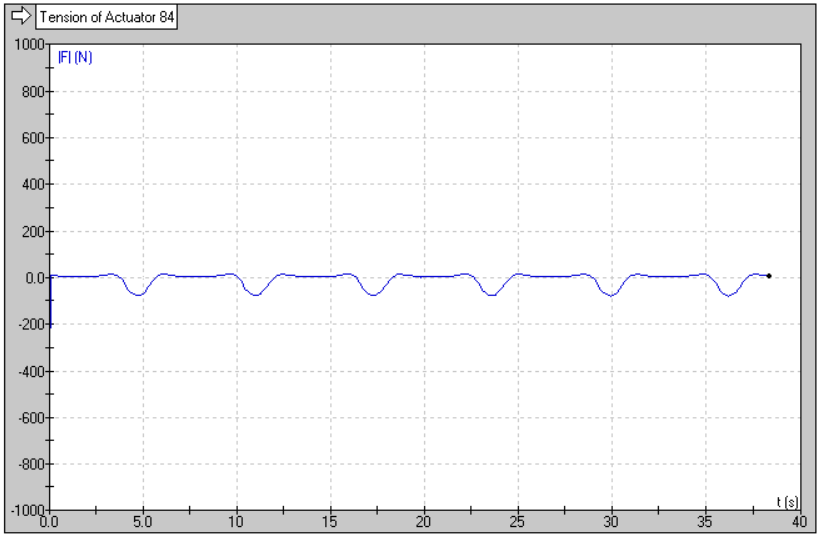
\includegraphics[width=0.7\linewidth]{Images/ac tension.png}
    \caption{Actuator tension}
\end{figure}

\begin{figure}[H]
    \centering
    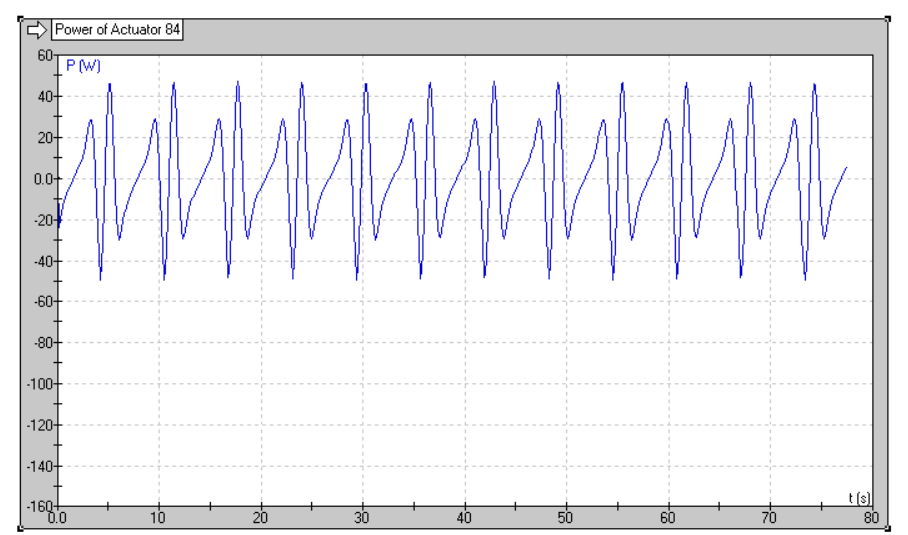
\includegraphics[width=0.7\linewidth]{Images/input power.png}
    \caption{input power}
\end{figure}

\begin{figure}[H]
    \centering
    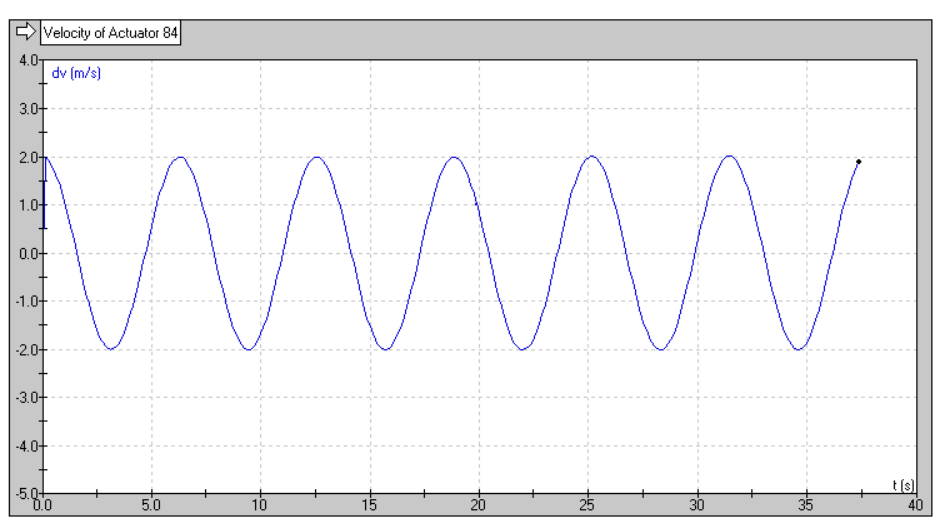
\includegraphics[width=0.7\linewidth]{Images/ac velocity.png}
    \caption{Actuator velocity}
\end{figure}

\begin{figure}[H]
    \centering
    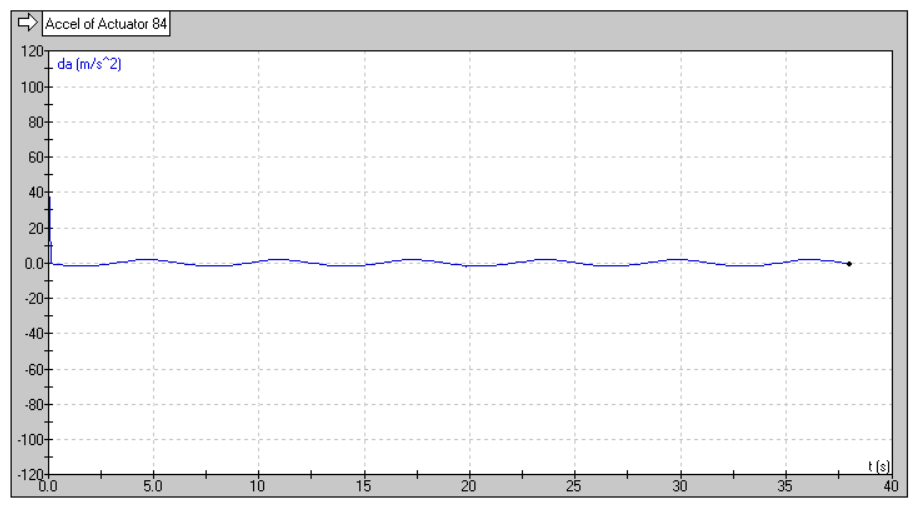
\includegraphics[width=0.7\linewidth]{Images/ac acc.png}
    \caption{Actuator acceleration}
\end{figure}

\begin{figure}[H]
    \centering
    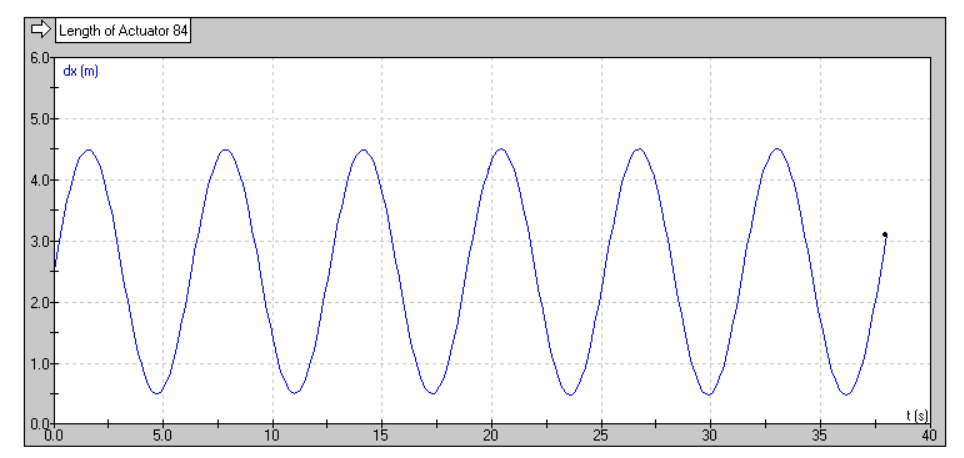
\includegraphics[width=0.7\linewidth]{Images/ac length.png}
    \caption{Actuator length}
\end{figure}

\begin{figure}[H]
    \centering
    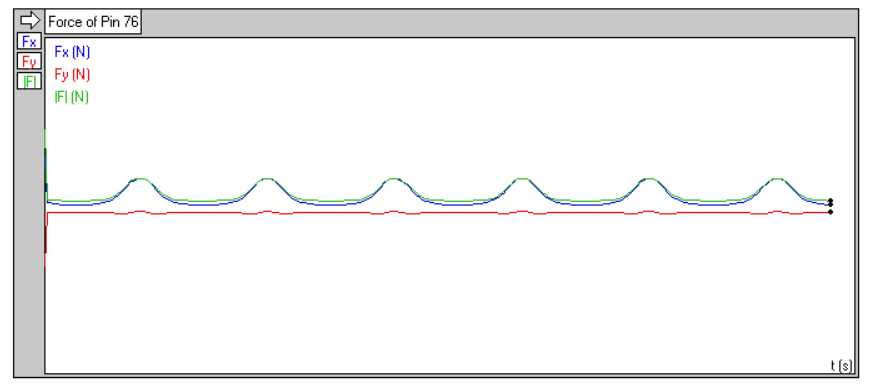
\includegraphics[width=0.7\linewidth]{Images/mem 10.png}
    \caption{Member 10 force}
\end{figure}

\begin{figure}[H]
    \centering
    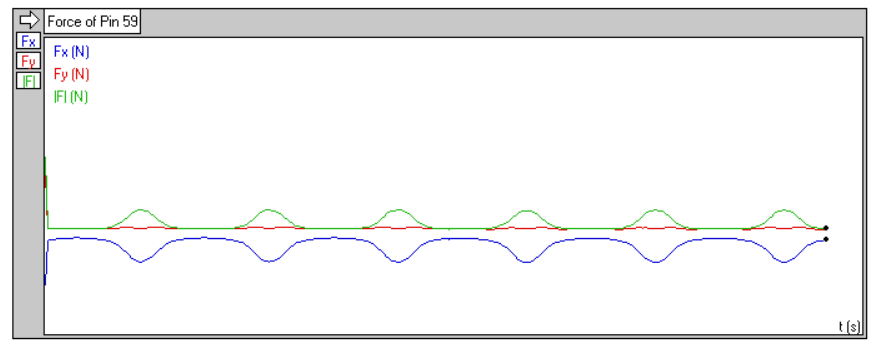
\includegraphics[width=0.7\linewidth]{Images/mem 12.png}
    \caption{Member 12 force}
\end{figure}

\begin{figure}[H]
    \centering
    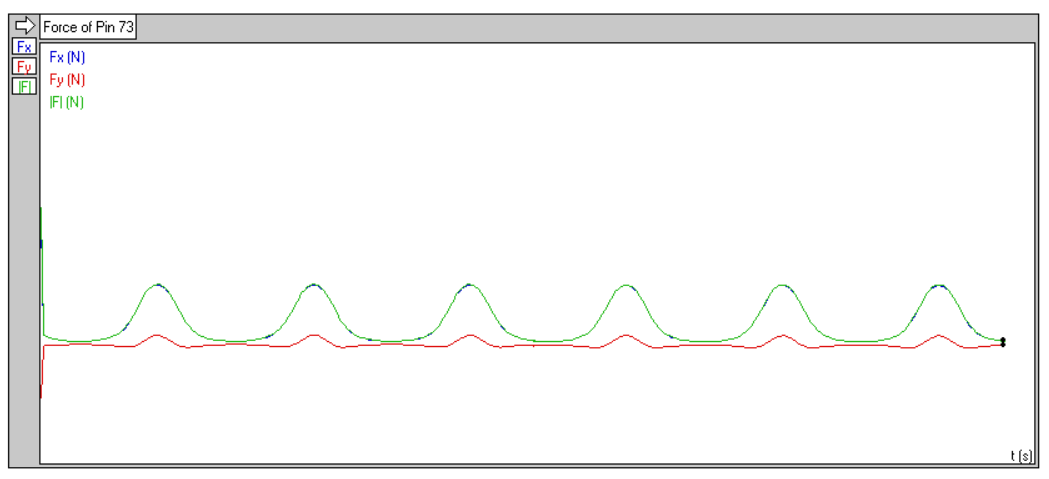
\includegraphics[width=0.7\linewidth]{Images/mem 11.png}
    \caption{Member 11 force}
\end{figure}

\begin{figure}[H]
    \centering
    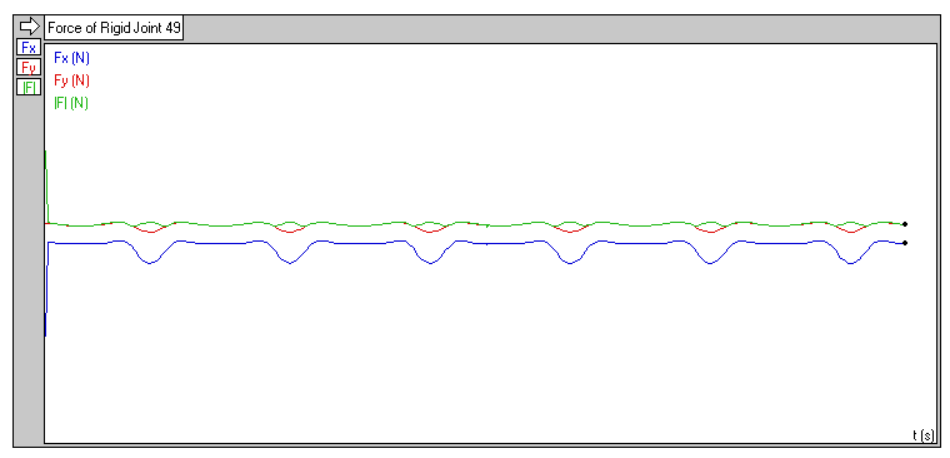
\includegraphics[width=0.7\linewidth]{Images/mem 13.png}
    \caption{Member 13 force}
\end{figure}

\begin{figure}[H]
    \centering
    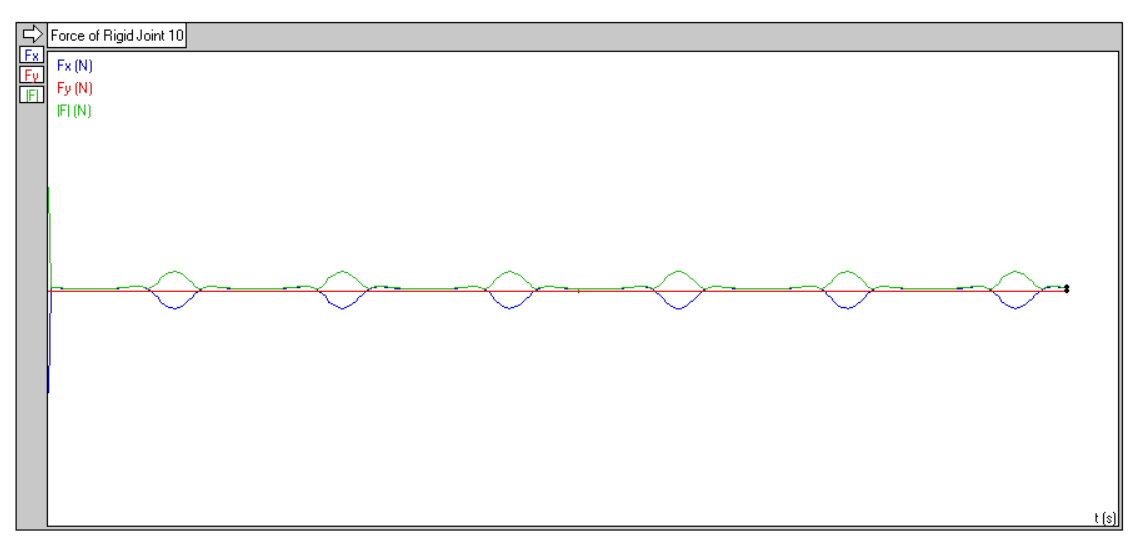
\includegraphics[width=0.7\linewidth]{Images/mem 15.png}
    \caption{Member 15 force}
\end{figure}

\begin{figure}[H]
    \centering
    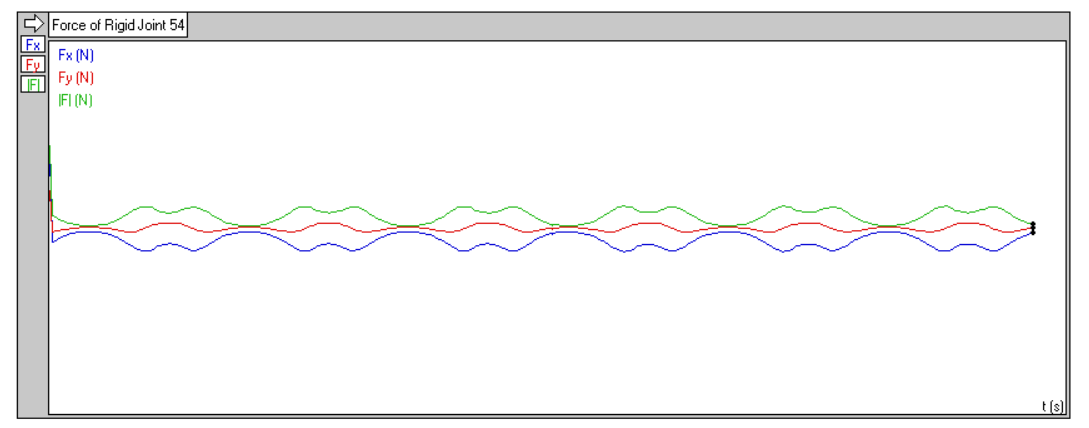
\includegraphics[width=0.7\linewidth]{Images/mem 16.png}
    \caption{Member 16 force}
\end{figure}

\newpage
\section*{Conclusion}
In conclusion, robot grippers are mainly used for their ability to perform routine actions tirelessly,
where a human would be more error-prone. For this reason, we've designed a robot gripper (albeit small-scale), 
which performs said menial tasks without any issues. With this report, we have included the necessary dimensions 
needed for the design, as well as the masses required to construct such a system, alongside some images
of the finished design.

\newpage
\section*{References}
$^{(1)}$ \href{https://www.universal-robots.com/in/blog/robotic-arm/}{Universal Robots. "ROBOTIC ARM"}
$^{(2)}$ \href{https://www.universal-robots.com/blog/robot-grippers-explained/}{Universal Robots. "Robot Grippers Explained"}
\end{document}